\documentclass{beamer}

\usetheme{Warsaw}

\definecolor{Indigo}{rgb}{0.18000, 0.00000, 0.50000}
\definecolor{PigeonBG}{rgb}{0.00000, 0.00000, 0.50000}

\usecolortheme[named=Indigo]{structure}
\setbeamercolor*{block title example}{fg=white, bg=PigeonBG}

\newcommand{\vs}{\\~\\}

% function restriction command
\newcommand{\restr}[2]{{\left.\kern-\nulldelimiterspace #1 \vphantom{\big|} \right|_{#2} }}
\newcommand{\N}{\mathbb{N}}
\newcommand{\RT}{\mathsf{RT}}
\newcommand{\red}{\mathsf{red}}
\newcommand{\blue}{\mathsf{blue}}

\title[Pigeon Hole Principle]{The Amazingly Useful Pigeon Hole Principle}
\author[]{Jared Corduan}
\date{February 1, 2018}

\usepackage{tikz}
\usepackage{verbatim}

\begin{document}

\begin{frame}
  \titlepage
\end{frame}

\begin{frame}
  These slides are available at:
  \url{https://github.com/JaredCorduan/pigeon-talk}
  \vs
  The code is available at:
  \url{https://github.com/JaredCorduan/ramsey}
\end{frame}

\begin{frame}{outline of this talk}
  \begin{itemize}
    \item the pigeon hole priciple is useful!
    \item its usefulness may be related to induction
    \item a constructive view of the (infinite) pigeon hole priciple
  \end{itemize}
\end{frame}

\begin{frame}{(Finite) Pigeon Hole Principle}
  \begin{definition}[Finite Pigeon Hole Principle]
    If $n$ items are put into $m$ containers, with $n > m$,
    then at least one container must contain more than one item.
  \end{definition}
\end{frame}

\begin{frame}{Finite Pigeon Hole Principle}
  \begin{theorem}[Fermat’s theorem on sums of two squares]
    For odd prime number p,
    $p=x^2+y^2$ if and only if $p \equiv 1 \mod 4$
  \end{theorem}

  \uncover<2->{
    The only if direction is straight-forward.

    Let $x^2 + 1 = 0 \mod p$ (by Euler's criterion)

  }
  \uncover<3->{
    Pigeons: all $(u, v)$ such that $0 \leq u,v < \sqrt{p}$

  }
  \uncover<4->{
    There are $(\lfloor \sqrt{p} \rfloor + 1)^2 > p$ pigeons.

  }
  \uncover<5->{
    Place pigeon $(u, v)$ into hole $ux-v \mod p$. There are $p$ holes.
  }
  \uncover<6->{
    \begin{equation*}
      \begin{array}{r@{~\equiv~}ll}
        u_1x-v_1 & u_2x-v_2 & \mod p \\
  }
  \uncover<7->{
        (u_1-u_2)^2x^2 & (v_1-v_2)^2 & \mod p \\
  }
  \uncover<8->{
        0 & (u_1-u_2)^2 + (v_1-v_2)^2 &  \mod p \\
      \end{array}
    \end{equation*}
  }
  \uncover<9->{
    \begin{equation*}
      0 < (u_1-u_2)^2 + (v_1-v_2)^2 < (\sqrt p)^2 + (\sqrt p)^2 = 2p
    \end{equation*}
  }
\end{frame}

\begin{frame}{Infinite Sets}
  ``In 1872 Dedekind was putting together \textit{Was sind und was sollen die Zahlen?},
  and he would be the first to define infinite set, with the definition
  being a set for which there is a one-to-one correspondence with a proper
  subset. This is just the negation of the Pigeonhole Principle.  Dedekind
  in effect had inverted a negative aspect of finite cardinality into a positive
  existence definition of the infinite''
  \vs
  -Akihiro Kanamori, \textit{The Mathematical Infinite as a Matter of Method}
\end{frame}

\begin{frame}{Infinite Pigeon Hole Principle}
  \begin{definition}[Infinite Pigeon Hole Principle]
    If infinitely many items are put into finitely many containers,
    then at least one container must contain infinitely many items.
  \end{definition}
\end{frame}

\begin{frame}{Infinite Ramsey's Theorem}

  \begin{theorem}[Infinite Ramsey's Theorem - $\RT^2_2$]
    Given a mapping $f:[\N]^2 \to \{\red, \blue\}$

    there is an infinite set $H\subseteq\N$ and a color $c \in \{\red, \blue\}$
    
    such that $\restr{f}{[H]^2}(x) = c$ for all $x\in H$.
  \end{theorem}

  \uncover<2->{
  \begin{theorem}[Infinite Ramsey's Theorem - $\mathsf{RT}^n_k$]
    For all $n,k\in\N$

    Given a mapping $f:[\N]^n \to \{1, \ldots, k\}$

    there is an infinite set $H\subseteq\N$ and a color $1 \leq c\leq k$

    such that $\restr{f}{[H]^n}(x) = c$ for all $x\in H$.
  \end{theorem}
  }
\end{frame}

\begin{frame}{Proof Infinite $\mathsf{RT}^2_2$}
  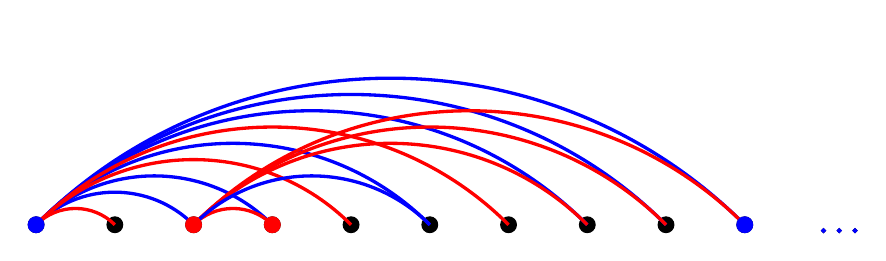
\begin{tikzpicture}
  \uncover<1->{
    \draw [fill] (0,0) circle [radius=0.1];
    \draw [fill] (9,0) circle [radius=0.1];

    \draw [fill] (10  ,-0.075) circle [radius=0.025];
    \draw [fill] (10.2,-0.075) circle [radius=0.025];
    \draw [fill] (10.4,-0.075) circle [radius=0.025];
  }
  \uncover<1-3>{
    \draw [fill] (1,0) circle [radius=0.1];
    \draw [fill] (4,0) circle [radius=0.1];
    \draw [fill] (6,0) circle [radius=0.1];
  }
  \uncover<1-6>{
    \draw [fill] (7,0) circle [radius=0.1];
    \draw [fill] (8,0) circle [radius=0.1];
  }
  \uncover<1-9>{
    \draw [fill] (2,0) circle [radius=0.1];
    \draw [fill] (3,0) circle [radius=0.1];
  }
  \uncover<1-5>{
    \draw [fill] (5,0) circle [radius=0.1];
  }
  \uncover<2-4>{
    \draw [blue, very thick] (0,0) to [out=45] (2,0);
    \draw [blue, very thick] (0,0) to [out=45] (3,0);
    \draw [blue, very thick] (0,0) to [out=45] (5,0);
    \draw [blue, very thick] (0,0) to [out=45] (7,0);
    \draw [blue, very thick] (0,0) to [out=45] (8,0);
    \draw [blue, very thick] (0,0) to [out=45] (9,0);
  }
  \uncover<2-3>{
    \draw [red, very thick] (0,0) to [out=45] (1,0);
    \draw [red, very thick] (0,0) to [out=45] (4,0);
    \draw [red, very thick] (0,0) to [out=45] (6,0);
  }
  \uncover<4->{
    \draw [blue, fill] (0,0) circle [radius=0.1];
  }
  \uncover<5-6>{
    \draw [red, very thick] (2,0) to [out=45] (3,0);
    \draw [red, very thick] (2,0) to [out=45] (7,0);
    \draw [red, very thick] (2,0) to [out=45] (8,0);
    \draw [red, very thick] (2,0) to [out=45] (9,0);
  }
  \uncover<5>{
    \draw [blue, very thick] (2,0) to [out=45] (5,0);
  }
  \uncover<6-9>{
    \draw [red, fill] (2,0) circle [radius=0.1];
  }
  \uncover<7-9>{
    \draw [red, fill] (3,0) circle [radius=0.1];
  }
  \uncover<8->{
    \draw [blue, fill] (9,0) circle [radius=0.1];
  }
  \uncover<10->{
    \draw [blue, fill] (10  ,-0.075) circle [radius=0.025];
    \draw [blue, fill] (10.2,-0.075) circle [radius=0.025];
    \draw [blue, fill] (10.4,-0.075) circle [radius=0.025];
  }
  \end{tikzpicture}
  \uncover<3-4>{
    \vs
    By the pigeon hole principle one color has infinitely many edges. Suppose blue is infinite.
  }
  \uncover<9->{
    \vs
    Use the pigeon hole principle one last time!
  }
\end{frame}

\begin{frame}{Partition Ordinals}
  Given a well-ordering $A$ and a coloring $f:A\to\{\mathsf{red}, \mathsf{blue}\}$,
  when is there an isomorphic copy of $A$ inside one of the colors?
  \vs
  Ordinals $\alpha$ with the property that every such coloring has
  an monocromatic copy of $\alpha$ are called partition ordinals.
  \vs
  Known examples are $\omega^n$ for $n\in\mathbb{N}$, and $\omega^{\omega}$.
\end{frame}

\begin{frame}{Partition Ordinals}
  Consider $\mathbb{N}\times\mathbb{N}$ ordered lexicographically:
  \vs~\\
  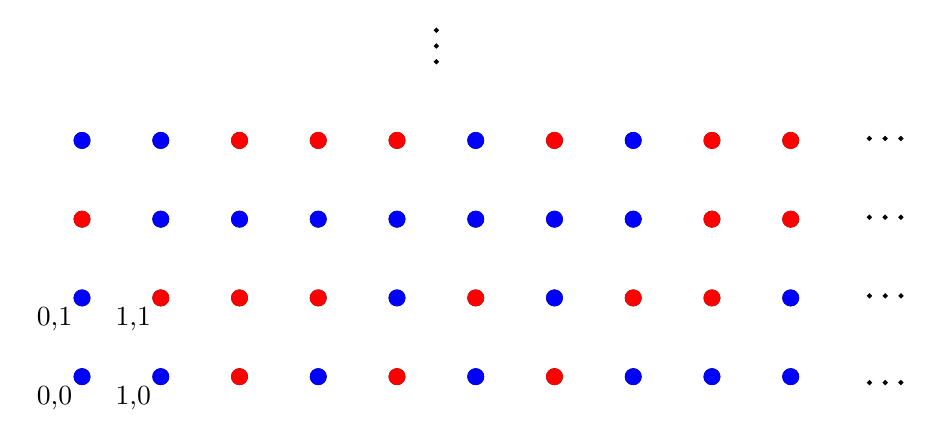
\begin{tikzpicture}
    \draw [fill] (0,0) circle [radius=0.1];
    \node [below left] at (0, 0) {0,0};
    \draw [fill] (1,0) circle [radius=0.1];
    \node [below left] at (1, 0) {1,0};
    \draw [fill] (2,0) circle [radius=0.1];
    \draw [fill] (3,0) circle [radius=0.1];
    \draw [fill] (4,0) circle [radius=0.1];
    \draw [fill] (5,0) circle [radius=0.1];
    \draw [fill] (6,0) circle [radius=0.1];
    \draw [fill] (7,0) circle [radius=0.1];
    \draw [fill] (8,0) circle [radius=0.1];
    \draw [fill] (9,0) circle [radius=0.1];

    \draw [fill] (10  ,-0.075) circle [radius=0.025];
    \draw [fill] (10.2,-0.075) circle [radius=0.025];
    \draw [fill] (10.4,-0.075) circle [radius=0.025];

    \draw [fill] (0,1) circle [radius=0.1];
    \node [below left] at (0, 1) {0,1};
    \draw [fill] (1,1) circle [radius=0.1];
    \node [below left] at (1, 1) {1,1};
    \draw [fill] (2,1) circle [radius=0.1];
    \draw [fill] (3,1) circle [radius=0.1];
    \draw [fill] (4,1) circle [radius=0.1];
    \draw [fill] (5,1) circle [radius=0.1];
    \draw [fill] (6,1) circle [radius=0.1];
    \draw [fill] (7,1) circle [radius=0.1];
    \draw [fill] (8,1) circle [radius=0.1];
    \draw [fill] (9,1) circle [radius=0.1];

    \draw [fill] (10  ,1.025) circle [radius=0.025];
    \draw [fill] (10.2,1.025) circle [radius=0.025];
    \draw [fill] (10.4,1.025) circle [radius=0.025];

    \draw [fill] (0,2) circle [radius=0.1];
    \draw [fill] (1,2) circle [radius=0.1];
    \draw [fill] (2,2) circle [radius=0.1];
    \draw [fill] (3,2) circle [radius=0.1];
    \draw [fill] (4,2) circle [radius=0.1];
    \draw [fill] (5,2) circle [radius=0.1];
    \draw [fill] (6,2) circle [radius=0.1];
    \draw [fill] (7,2) circle [radius=0.1];
    \draw [fill] (8,2) circle [radius=0.1];
    \draw [fill] (9,2) circle [radius=0.1];

    \draw [fill] (10  ,2.025) circle [radius=0.025];
    \draw [fill] (10.2,2.025) circle [radius=0.025];
    \draw [fill] (10.4,2.025) circle [radius=0.025];

    \draw [fill] (0,3) circle [radius=0.1];
    \draw [fill] (1,3) circle [radius=0.1];
    \draw [fill] (2,3) circle [radius=0.1];
    \draw [fill] (3,3) circle [radius=0.1];
    \draw [fill] (4,3) circle [radius=0.1];
    \draw [fill] (5,3) circle [radius=0.1];
    \draw [fill] (6,3) circle [radius=0.1];
    \draw [fill] (7,3) circle [radius=0.1];
    \draw [fill] (8,3) circle [radius=0.1];
    \draw [fill] (9,3) circle [radius=0.1];

    \draw [fill] (10  ,3.025) circle [radius=0.025];
    \draw [fill] (10.2,3.025) circle [radius=0.025];
    \draw [fill] (10.4,3.025) circle [radius=0.025];

    \draw [fill] (4.5,4) circle [radius=0.025];
    \draw [fill] (4.5,4.2) circle [radius=0.025];
    \draw [fill] (4.5,4.4) circle [radius=0.025];

  \uncover<2>{
    \draw [fill, blue] (0,0) circle [radius=0.1];
    \draw [fill, blue] (1,0) circle [radius=0.1];
    \draw [fill, red] (2,0) circle [radius=0.1];
    \draw [fill, blue] (3,0) circle [radius=0.1];
    \draw [fill, red] (4,0) circle [radius=0.1];
    \draw [fill, blue] (5,0) circle [radius=0.1];
    \draw [fill, red] (6,0) circle [radius=0.1];
    \draw [fill, blue] (7,0) circle [radius=0.1];
    \draw [fill, blue] (8,0) circle [radius=0.1];
    \draw [fill, blue] (9,0) circle [radius=0.1];

    \draw [fill, blue] (0,1) circle [radius=0.1];
    \draw [fill, red] (1,1) circle [radius=0.1];
    \draw [fill, red] (2,1) circle [radius=0.1];
    \draw [fill, red] (3,1) circle [radius=0.1];
    \draw [fill, blue] (4,1) circle [radius=0.1];
    \draw [fill, red] (5,1) circle [radius=0.1];
    \draw [fill, blue] (6,1) circle [radius=0.1];
    \draw [fill, red] (7,1) circle [radius=0.1];
    \draw [fill, red] (8,1) circle [radius=0.1];
    \draw [fill, blue] (9,1) circle [radius=0.1];

    \draw [fill, red] (0,2) circle [radius=0.1];
    \draw [fill, blue] (1,2) circle [radius=0.1];
    \draw [fill, blue] (2,2) circle [radius=0.1];
    \draw [fill, blue] (3,2) circle [radius=0.1];
    \draw [fill, blue] (4,2) circle [radius=0.1];
    \draw [fill, blue] (5,2) circle [radius=0.1];
    \draw [fill, blue] (6,2) circle [radius=0.1];
    \draw [fill, blue] (7,2) circle [radius=0.1];
    \draw [fill, red] (8,2) circle [radius=0.1];
    \draw [fill, red] (9,2) circle [radius=0.1];

    \draw [fill, blue] (0,3) circle [radius=0.1];
    \draw [fill, blue] (1,3) circle [radius=0.1];
    \draw [fill, red] (2,3) circle [radius=0.1];
    \draw [fill, red] (3,3) circle [radius=0.1];
    \draw [fill, red] (4,3) circle [radius=0.1];
    \draw [fill, blue] (5,3) circle [radius=0.1];
    \draw [fill, red] (6,3) circle [radius=0.1];
    \draw [fill, blue] (7,3) circle [radius=0.1];
    \draw [fill, red] (8,3) circle [radius=0.1];
    \draw [fill, red] (9,3) circle [radius=0.1];
  }
  \end{tikzpicture}
\end{frame}

\begin{frame}{Finite Ramsey's Theorem}
  \begin{definition}
    We write
    $$n\to(h)^k_r$$
    to mean that for every $r$-coloring of $\{1, 2, \ldots, n\}^k$,
    there is a set $H\subseteq\{1, 2, \ldots, k\}$ such that $|H|=h$ and a color $c$
    such that $H^k$ is colored $c$.
  \end{definition}

  \uncover<2->{
    \begin{example}
      $6\to(3)^2_2$
    \end{example}
  }
  \uncover<3->{
    \begin{tikzpicture}
      \draw [fill] (0,1) circle [radius=0.1];
      \draw [fill] (1,0) circle [radius=0.1];
      \draw [fill] (2,2) circle [radius=0.1];
      \draw [fill] (3,0) circle [radius=0.1];
      \draw [fill] (4,1) circle [radius=0.1];
      \draw [fill] (6,2) circle [radius=0.1];

      \draw [red, very thick] (0,1) to (1,0);
      \draw [red, very thick] (0,1) to (2,2);
      \draw [blue, very thick] (0,1) to (3,0);
      \draw [blue, very thick] (0,1) to (4,1);
      \draw [blue, very thick] (1,0) to (2,2);
      \draw [red, very thick] (1,0) to (3,0);
      \draw [blue, very thick] (1,0) to (4,1);
      \draw [blue, very thick] (2,2) to (3,0);
      \draw [red, very thick] (2,2) to (4,1);
      \draw [red, very thick] (3,0) to (4,1);
    }

  \uncover<4->{
      \draw (6,2) to (0,1);
      \draw (6,2) to (1,0);
      \draw (6,2) to (2,2);
      \draw (6,2) to (3,0);
      \draw (6,2) to (4,1);
    \end{tikzpicture}
  }
\end{frame}

\begin{frame}{Finite Ramsey's Theorem}
  \begin{theorem}[Finite Ramsey's Theorem]
    For every $k, h, r\in\mathbb{N}$ there is $n\in\mathbb{N}$ such that
    if $n_0 \geq n$ then $n_0 \to (h)^k_r$
  \end{theorem}

  \uncover<2->{ Proof: by compactness!}
  \uncover<3->{ (We'll see if we have time for the proof.) }
\end{frame}

\begin{frame}{Finite Ramsey's Theorem}
  Suppose aliens invade the earth and threaten to obliterate it in a year's
  time unless human beings can find the Ramsey number for red five and blue five.
  We could marshal the world's best minds and fastest computers, and within a
  year we could probably calculate the value. If the aliens demanded the Ramsey
  number for red six and blue six, however, we would have no choice but to launch
  a preemptive attack.
  \vs
  - Paul Erd\H{o}s, $\sim$ 1990.
\end{frame}

\begin{frame}{Bounding and Induction}
  Consider these induction and induction-like axioms:
  \vs
  successor induction:
  \begin{equation*}
    \varphi(0) \land (\forall x)(\varphi(x) \to \varphi(x+1)) \to (\forall x)\varphi(x)
  \end{equation*}
  \uncover<2->{
    order induction:
    \begin{equation*}
      (\forall x)[((\forall y < x)\varphi (y)) \to \varphi (x)] \to (\forall x)\varphi(x)
    \end{equation*}
  }
  \uncover<3->{
    least number:
    \begin{equation*}
      (\exists x)\varphi(x) \to (\exists x)(\varphi(x) \land (\forall y < x)\neg\varphi(y))
    \end{equation*}
  }
  \uncover<4->{
    bounding:
    \begin{equation*}
      (\forall u)[(\forall x\leq u)(\exists y)\varphi(x, y)
      \to (\exists v)(\forall x \leq u)(\exists y \leq v)\varphi(x, y)]
    \end{equation*}
  }
\end{frame}

\begin{frame}{The arithmetic heirarchy}
  In Peano Arithmetic, we write:

  $(\forall x \leq y)\varphi$ as shorthand for $(\forall x)(x \leq y \to \varphi)$
  , and

  $(\exists x \leq y)\varphi$ as shorthand for $(\exists x)(x \leq y \land \varphi)$.
  \vs
  A formula is said to be bounded, or $\Sigma_0$, or $\Pi_0$, if it contains
  only bounded quantifiers.
  \vs
  \uncover<2->{
    A $\Sigma_1$ formula has the form $(\exists x) \varphi$ for a bounded formula $\varphi$.

  }
  \uncover<3->{

    A $\Pi_1$ formula has the form $(\forall x) \varphi$ for a bounded formula $\varphi$.
  }
  \uncover<4->{

    A $\Sigma_2$ formula has the form $(\exists x)(\forall y) \varphi$ for a bounded formula $\varphi$.
  }
  \uncover<5->{

    A $\Pi_2$ formula has the form $(\forall x)(\exists y) \varphi$ for a bounded formula $\varphi$.
  }
\end{frame}

\begin{frame}{Peano Arithmetic with restricted Induction}
  Peano arithmetic with the full induction axioms replaced by:
  \begin{itemize}
    \item successor induction for $\Sigma_n$ formulas: $\mathsf{I}\Sigma_n$.
    \item order induction for $\Sigma_n$ formulas: $\mathsf{I}'\Sigma_n$.
    \item least number axiom for $\Sigma_n$ formulas: $\mathsf{L}\Sigma_n$.
    \item bounding axioms for $\Sigma_n$ formulas: $\mathsf{B}\Sigma_n$.
    \item \ldots $\Pi_n$ \ldots
  \end{itemize}
\end{frame}

\begin{frame}{Peano Arithmetic with restricted Induction}
  \begin{theorem}
    For each $n\in\mathbb{N}$,
    the following theories are equivalent:

    $\mathsf{I}\Sigma_n$,
    $\mathsf{I}\Pi_n$,
    $\mathsf{I}'\Sigma_n$,
    $\mathsf{I}'\Pi_n$,
    $\mathsf{L}\Sigma_n$,
    $\mathsf{L}\Pi_n$
  \end{theorem}

  \begin{theorem}
    For each $n\in\mathbb{N}$,
    the following theories are equivalent:

    $\mathsf{B}\Sigma_{n+1}$,
    $\mathsf{B}\Pi_n$,
    $\mathsf{L}\Delta_{n+1}$,
  \end{theorem}

\end{frame}

\begin{frame}{Finite PHP in Peano Arithmetic}
  Let $\mathsf{PHP}$ be the statement that

 ``$\varphi$ does not define a one-one mapping of $u$ onto $u+1$".
 \vs
 \begin{theorem}
   For each $n\geq 2$,
   the following theories are equivalent:
   $\mathsf{PHP}\Sigma_{n}$,
   $\mathsf{B}\Sigma_{n}$
   \vs
   (And $\mathsf{PHP}\Sigma_{1}~\implies~\mathsf{B}\Sigma_{1}$.)
 \end{theorem}
\end{frame}

\begin{frame}{Reference for these fragments of arithmetic}
  \begin{center}
  A great reference for these restricted theories is:
  \vs
  ``Metamathematics of First-Order Arthimetic"
  \\
  by H\'ajek and Pudl\'ak.
  \end{center}
\end{frame}

\begin{frame}{Infinite PHP in Second-Order Arithmetic}
  \begin{theorem}[Jeff Hirst, 1987]
   The following are equivalent (over $\mathsf{RCA}_0$):

   $\mathsf{PHP}$,
   $\mathsf{B}\Pi^0_{2}$

 \end{theorem}
\end{frame}

\begin{frame}{Pigeon Hole Principle is not constructive}
  The inifinite pigeon hole principle fails to hold constructively (in the sense of intuitionism).
  \vs
  This was studied by Veldman and Bezem in
  ``Ramsey's theorem and the pigeonhole principle in intuitionistic mathematics".
  \vs
  \uncover<2->{
    Pick your favorite sequence of digits and color $n$ with $\red$ if
    this sequence appears in the first $n$ decimals of $\pi$. Color it $\blue$ otherwise.
  }
\end{frame}

\begin{frame}{A constructive pigeon hole principle}
  \begin{theorem}
    The intersection of two cofinite sets is cofinite.
  \end{theorem}
  \uncover<2->{
    \begin{definition}[almost full]
      Let $Y: (\N\to\N) \to \N$.
      We say that $A\subseteq\N$ is \textbf{almost full for $Y$}
      if given any increasing $f:\N\to\N$, $f(Y(f))\in A$.
      \\
      We say that $A\subseteq\N$ is \textbf{almost full}
      if it is almost full for some $Y$.
    \end{definition}
  Note that this definition is classically equivalent to being cofinite.
}
  \uncover<3->{
    \begin{theorem}
      The intersection of two almost full sets is almost full.
    \end{theorem}
  }
\end{frame}

\begin{frame}{A constructive pigeon hole principle in Lean}
Now we look at \url{https://github.com/JaredCorduan/ramsey}.
\end{frame}

\begin{frame}{Compactness - fun tangent}
  \begin{theorem}[Godel, 1929]
    Every finitely satisfiable set of sentences
    (in a countable first-order formal language) is satisfiable.
  \end{theorem}
  This is often call the compactess theorem,
  since it asserts that the following topological space is compact:
  \uncover<2->{
    \begin{itemize}
      \item A point in the space is a complete theory $T$ in the language $L$.
      \item The basis for the topology has the open sets $U(\sigma) = \{T: \sigma\in T\}$
        for every sentence $\sigma$ of $L$.
    \end{itemize}
  }
\end{frame}

\begin{frame}{Proof of finite Ramsey - fun tangent}
  If Ramsey's theorem failed there would be $k, r, h\in\N$ such that:

  For all $b$, there is a set $X$ of size at least $b$ and there is an
    $r$-coloring of $X$ in $k$ colors with no monochromatic subset $H\subseteq X$ of size h.

    \uncover<2->{
      Let $\psi(\vec{x})$ be a formula specifying a coloring of $\vec{x}$.

    }
    \uncover<3->{
    Let $\phi(\vec{x})$ be a formula saying that no $h$-element subset of
    $\vec{x}$ is monochromatic.

    }

    \uncover<4->{
    Let $\sigma_b$ be a formula saying that there are at least $b$-many elements.

    }

    \uncover<5->{
    Then $\Gamma_b = \{\psi, \phi, \sigma_0, \sigma_1, \ldots, \sigma_b\}$ is satisfiable.

    }

    \uncover<6->{
    By compactness, then so is $\Gamma = \{\psi, \phi, \sigma_0, \sigma_1, \ldots\}$.

    }

    \uncover<7->{
    But this contradicts the infinite pigeon hold priciple!

    }

    \uncover<8->{
    See
    \url{https://math.dartmouth.edu/archive/m69w13/public_html/m69examplepaper3ramseyWEB.pdf}
    for the full details.
    }
\end{frame}

\begin{frame}
  \centering
  thank you for listening!
\end{frame}

\end{document}
